\documentclass[tikz,border=5pt]{standalone}
\usepackage{tikz}
\usetikzlibrary{positioning,fit,backgrounds,calc,shapes.geometric}
\usepackage{graphicx}
\usepackage{xcolor}

\definecolor{gitopsblue}{RGB}{51,108,229}
\definecolor{manualgray}{RGB}{102,102,102}
\definecolor{driftred}{RGB}{229,115,115}
\definecolor{warnorange}{RGB}{255,167,38}
\definecolor{okgreen}{RGB}{76,175,80}

\begin{document}
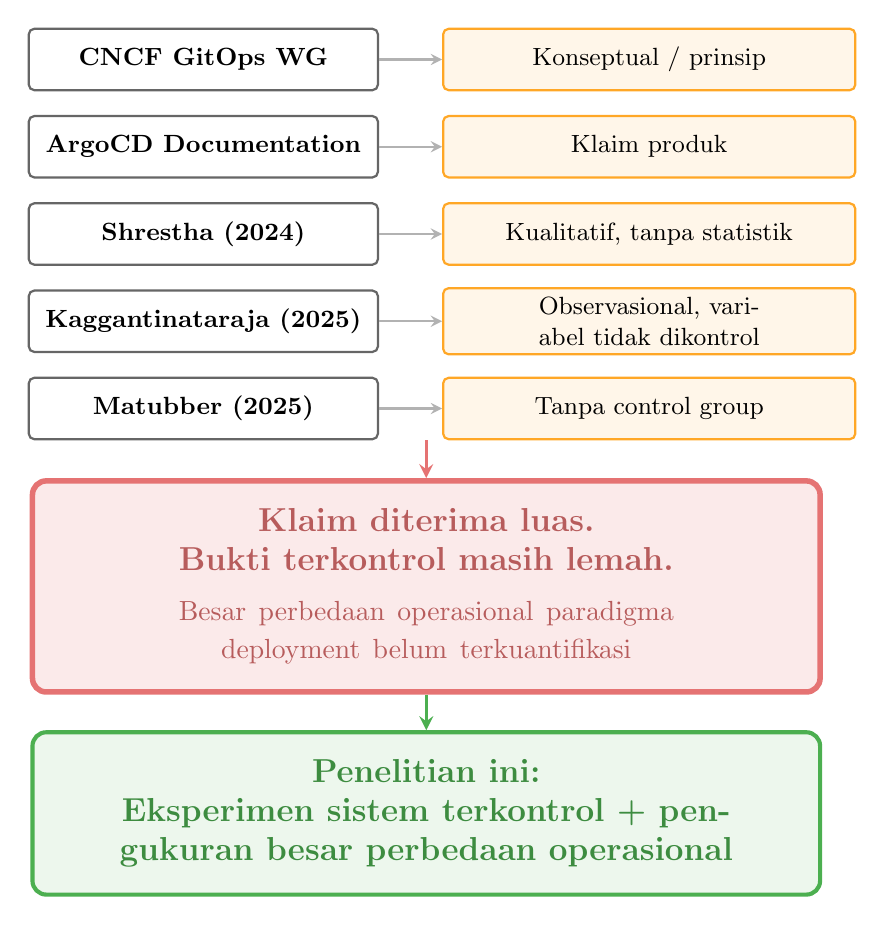
\begin{tikzpicture}[
    node distance=0.34cm,
    claim/.style={rectangle, rounded corners=2pt, draw=manualgray, fill=white,
                  text width=4.2cm, minimum height=0.78cm, align=center,
                  line width=0.8pt, font=\small\bfseries},
    evidence/.style={rectangle, rounded corners=2pt, draw=warnorange, fill=warnorange!10,
                     text width=5.0cm, minimum height=0.78cm, align=center,
                     line width=0.8pt, font=\small},
    gapbox/.style={rectangle, rounded corners=5pt, draw=driftred, fill=driftred!15,
                   inner sep=10pt, line width=2pt},
    arrow/.style={->, >=stealth, line width=0.8pt, draw=manualgray!50}
]

\node[claim] (s1) {CNCF GitOps WG};
\node[claim, below=0.3cm of s1] (s2) {ArgoCD Documentation};
\node[claim, below=0.3cm of s2] (s3) {Shrestha (2024)};
\node[claim, below=0.3cm of s3] (s4) {Kaggantinataraja (2025)};
\node[claim, below=0.3cm of s4] (s5) {Matubber (2025)};

\node[evidence, right=0.8cm of s1] (e1) {Konseptual / prinsip};
\node[evidence, right=0.8cm of s2] (e2) {Klaim produk};
\node[evidence, right=0.8cm of s3] (e3) {Kualitatif, tanpa statistik};
\node[evidence, right=0.8cm of s4] (e4) {Observasional, variabel tidak dikontrol};
\node[evidence, right=0.8cm of s5] (e5) {Tanpa control group};

\draw[arrow] (s1) -- (e1);
\draw[arrow] (s2) -- (e2);
\draw[arrow] (s3) -- (e3);
\draw[arrow] (s4) -- (e4);
\draw[arrow] (s5) -- (e5);

\node[gapbox, below=0.48cm of $(s5.south)!0.5!(e5.south)$, text width=9.3cm, align=center, font=\large\bfseries, text=driftred!80!black] (gap) {
    Klaim diterima luas.\\
    Bukti terkontrol masih lemah.\\[4pt]
    \normalfont\normalsize Besar perbedaan operasional paradigma deployment belum terkuantifikasi
};

\draw[->, >=stealth, line width=1.2pt, draw=driftred] ($(s5.south)!0.5!(e5.south)$) -- (gap);

\node[rectangle, rounded corners=5pt, draw=okgreen, fill=okgreen!10,
      inner sep=10pt, line width=1.5pt, below=0.45cm of gap,
       text width=9.3cm, align=center, font=\large\bfseries, text=okgreen!80!black] (ours) {
     Penelitian ini:\\
     Eksperimen sistem terkontrol + pengukuran besar perbedaan operasional
};

\draw[->, >=stealth, line width=1.2pt, draw=okgreen] (gap) -- (ours);

\end{tikzpicture}
\end{document}
